\setcounter{secnumdepth}{5}

\chapter{Scanning e DDoS}


\section{Scanning}
Lo scanning non è altro che un'ispezione molto oculata del \textbf{perimetro} di un'organizzazione o, più in generale, di una rete al fine di \textbf{individuare potenziali punti di accesso ai sistemi} del \textit{target}. Lo scanning è un'attività che viene a valle del \textit{footprinting} che invece permette il riconoscimento della rete. 
\newline La prima cosa, nello scanning, è quella di andare a \textbf{riconoscere} quali sono gli \textit{indirizzi IP} disponibili ed \textit{attivi} all'interno della rete. Per poter fare ciò, può essere utile contattarli ed attendere una risposta:
\begin{itemize}
    \item \textbf{La risposta arriva:} un nodo con quell'\textit{indirizzo IP} è attivo
    \item \textbf{La risposta non arriva:} non vi sono nodi attivi con quell' \textit{indirizzo IP}
\end{itemize}

Successivamente, è possibile verificare, sempre attraverso l'invio di pacchetti e alla risposta ottenuta, se sono presenti firewall con delle regole di filtraggio che dovrebbero essere aggirate. Per ultimo, ma non per importanza, attraverso lo \textbf{scanning} è possibile mantenere o meno l'anonimato a seconda delle tecniche di monitoraggio utilizzate. \newline Il monitoraggio può essere:
\begin{itemize}
    \item \textbf{Monitoraggio attivo:} prevede l'invio di pacchetti nella rete e un controllo delle risposte per verificare la presenza o meno di nodi attivi. Questo tipo di monitoraggio, essendo attivo, può essere più semplice da scovare
    \item \textbf{Monitoraggio passivo:} tecniche di ascolto senza invio di pacchetti nella rete che permettono di mantenere l'anonimato. 
\end{itemize}

È possibile effettuare lo scanning sia su \textbf{TCP} che su \textbf{UDP}. È ben noto che le porte sono $65'000$ ma alcune sono solo utilizzate solo su TCP, altre solo su UDP, altre per entrambe. 


\subsection{TCP Scan}
Lo scan over TCP è utile per scoprire quali sono le porte aperte di un dato indirizzo IP. In particolare, esso è necessario per lo scanning di tutte quelle porte che sono attive solo su TCP, quali: Porta 23 (Telnet), 25 (SMTP), 80 (HTTP), etc. 

\subsection{Pacchetto TCP}
La parte importante per lo scanning è l'Header del pacchetto TCP che si presenta come in foto. Oltre a dati quali porta sorgente e destinazione e il sequence number, sono presenti le "flags".

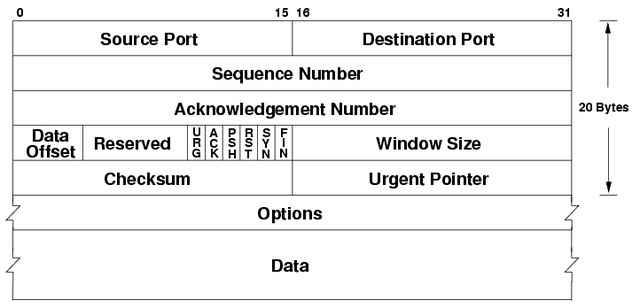
\includegraphics[scale=0.6]{UNINA_MSc_Thesis_Project/img/TCP_header.png}

Flags presenti header TCP, utili per alcune tecniche di scanning :
\begin{itemize}
%    \item CWR: gestione finestra di congestione
%    \item ECE: indica, se pari a 1, che l'host supporta ECN durante il 3WHS 
    \item URG: indica, se pari a 1, che sono presenti dati urgenti
    \item ACK: indica, se pari a 1, che il campo Acknowledgment number valido
    \item PSH: indica, se pari a 1, che i dati in arrivo non devono essere bufferizzati
    \item RST: indica, se pari a 1, che la connessione non è valida
    \item SYN: indica, se pari a 1, che l'host mittente vuole aprire una connessione TCP con il destinatario e specifica nel campo \textit{SN (Sequence Number)} il valore dell'\textit{Initial Sequence Number (ISN)}. Questo ha lo scopo di \textbf{sincronizzare} i numeri di sequenza dei due host. L'host che ha inviato il SYN deve attendere dall'host remoto un pacchetto SYN/ACK e, per avviare la connessione, deve inviare un "ACK".
    \item FIN: indica, se pari a 1, che l'host mittente del segmento vuole chiudere la connessione TCP aperta con l'host destinatario. Il mittente attende la conferma dal ricevente (con un FIN-ACK). A questo punto la connessione è ritenuta chiusa per metà: l'host che ha inviato FIN non potrà più inviare dati, mentre l'altro host ha il canale di comunicazione ancora disponibile. Quando anche l'altro host invierà il pacchetto con FIN impostato, la connessione, dopo il relativo FIN-ACK, sarà considerata completamente chiusa.
\end{itemize}

\subsubsection{SYN Scan}
Con questo tipo di scansione la connessione non viene mai attivata in quanto l'attaccante non procede mai con l'invio dell'ACK; per questo motivo, tale scansione è detta \textit{"Half-Opening scanning"}. Il SYN scan è una scansione che prevede l'invio di un pacchetto con il flag $SYN=1$ ed attende la ricezione di un $SYN-ACK$: se questo arriva, allora la porta è \textbf{aperta}; viceversa, se non arriva alcun $SYN-ACK$ la porta è \textbf{chiusa}. 

\subsubsection{FIN Scan}
Simile al SYN scan ma invia i pacchetti con flag $FIN=1$. Queste tecniche sono semplici ma meno utilizzate in quanto, in risposta a questi pacchetti TCP, possiamo avere dei comportamenti diversi a seconda del Sistema Operativo:
\begin{itemize}
    \item Specifica RFC793: 
    \begin{itemize}
        \item \textbf{Porta aperta:} Il pacchetto viene ignorato
        \item \textbf{Porta chiusa:} Viene inviato un pacchetto "RST"
    \end{itemize}
    \item Altro (ad es. Windows): rispondono inviando, in qualsiasi caso, un pacchetto TCP con flag RST attivo rendendo la scansione inefficace.
\end{itemize}

\subsection{XMASTree Scan}
Come il FIN scan ma invia i pacchetti con flag $FIN,URG,PUSH=1$. 

\subsection{UDP Scan}
L'UDP scan è una scansione utilizzata per rilevare quali sono i servizi attivi sul protocollo UDP. Normalmente gli UDP scan inviano pacchetti alle porte di un indirizzo IP da testare:
\begin{itemize}
    \item Nessun pacchetto risposta: porta chiusa
    \item Pacchetto ICMP type 3 - codice 3: porta chiusa
    \item Pacchetto ICMP type 3 - codice 1,2,9,10,13: pacchetto filtrato 
    \item Pacchetto di risposta: porta aperta 
\end{itemize}

\section{DoS}
Il Denial of Services è un attacco informatico che va a colpire la disponibilità di una risorsa all'interno di un sistema. In pratica, esso interrompe temporaneamente i servizi di un host connesso a una rete. Il Denial of Service si genera inondando il server con un numero elevato di richieste al fine di sovraccaricare i sistemi.

\section{DDoS}
Gli attacchi DDoS (Distributed Denial of Services) sono un tipo di attacco DoS che prevedono la creazione di una botnet, ovvero una rete di computer infettati che possono contattare un nodo remoto per effettuare attacchi informatici. Gli attacchi DDoS sofisticati sfruttano, in primo luogo, il modo in cui i protocolli eseguiti sui dispositivi odierni sono stati progettati per funzionare.

\subsection{Mirai Botnet Attack}
Il Mirai Botnet Attack è stato un attacco DDoS noto a partire dal 2016. Esso infetta dispositivi, li inserisce all'interno di una botnet per poi sferrare l'attacco. 

\subsubsection{Funzionamento: attacco a dizionario}
Il Mirai sfrutta tre componenti principali:
\begin{itemize}
    \item Virus: Il codice che cerca nuovi dispositivi IoT da infettare e compromettere per inserirli all'interno della botnet 
    \item CnC: Supporta un'interfaccia a riga di comando che permette, al Loader/Scanner di specificare a chi inviare l'attacco. In particolare, quando un dispositivo viene infettato, esso invia il proprio IP al CnC che si occuperà di inviarlo al Loader
    \item Loader/Scanner: si occupa di infettare il primo bot da cui parte la botnet e di caricare, sotto istruzioni del CnC, il malware sui nuovi bot vulnerabili scovati in rete. 
\end{itemize}

I passi del funzionamento sono mostrati in figura:

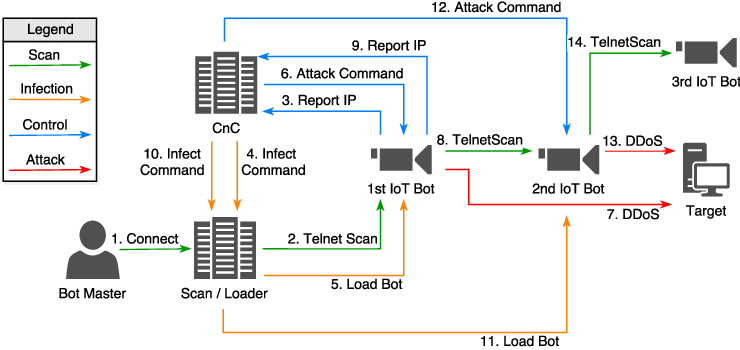
\includegraphics[scale=0.4]{UNINA_MSc_Thesis_Project/img/Mirai-Botnet-Infection-Methodology.png}

Il tipo di attacco Mirai sfrutta vulnerabilità del protocollo Telnet (porta 23 o 2323) su TCP. La vulnerabilità sfruttata è legata a:
\begin{itemize}
    \item Porta 23 aperta (Telnet)
    \item User e Password lasciati di default 
\end{itemize}
Ciò è possibile poiché, se username e password sono lasciati di default, si fa uso di un \textbf{dizionario} (attacco a dizionario: \textit{bruteforce}) contenente tutti i possibili user e password di "default" quali, ad esempio, root-root, admin-admin, root-admin, etc. per tentare di effettuare il login. In caso di login riuscito, il nuovo computer può essere considerato come nuovo bot della rete. 
